% Compiling with
% latexmk -halt-on-error -shell-escape -synctex=1 -pdf maths.tex
% (Recommend using a latexmkrc file so as just to run latexmk -pvc, for example)
% Probably you can achieve the same with an inordinate number of invocations of
% pdflatex -halt-on-error -shell-escape -synctex=1 maths.tex

% fleqn aligns equations to the left, a4 paper size, 11pt font, article class
\documentclass[fleqn,a4paper,11pt]{article}
\title{IA Vectors and Matrices Example Sheet 1, Revised Edition}
\author{Izaak van Dongen (\texttt{imv26})}

\usepackage{mymaths}
\usepackage{mystyle}

\begin{document}
 \maketitle\thispagestyle{empty} % no page number under title

 \begin{enumerate}
  \item
   Have
   \begin{align*}
    \abs{z - (1 + i)} &< 1
    \intertext{
     So then using the triangle inequalities for \(\abs{z_1 + z_2}\) and
     \(\abs{z_1 - z_2}\),}
    \abs{z - 3} &=   \abs{z - (1 + i) + (-2 + i)} \\
                &\le \abs{z - (1 + i)} + \abs{-2 + i} \\
                &<   1 + \sqrt 5 \\
    \text{and}\quad
    \abs{z - 3} &=   \abs{z - (1 + i) - (2 - i)} \\
                &\ge \abs[\Big]{\abs{z - (1 + i)} - \abs{2 - i}} \\
                &>   \abs[\Big]{1 - \sqrt 5} \quad
                     \text{picking \(\abs{z - (1 + i)}\) to be as close to
                           \(\sqrt 5\) as possible} \\
                &=   \sqrt 5 - 1
   \end{align*}
   \begin{figure}[H]
    \begin{center}
     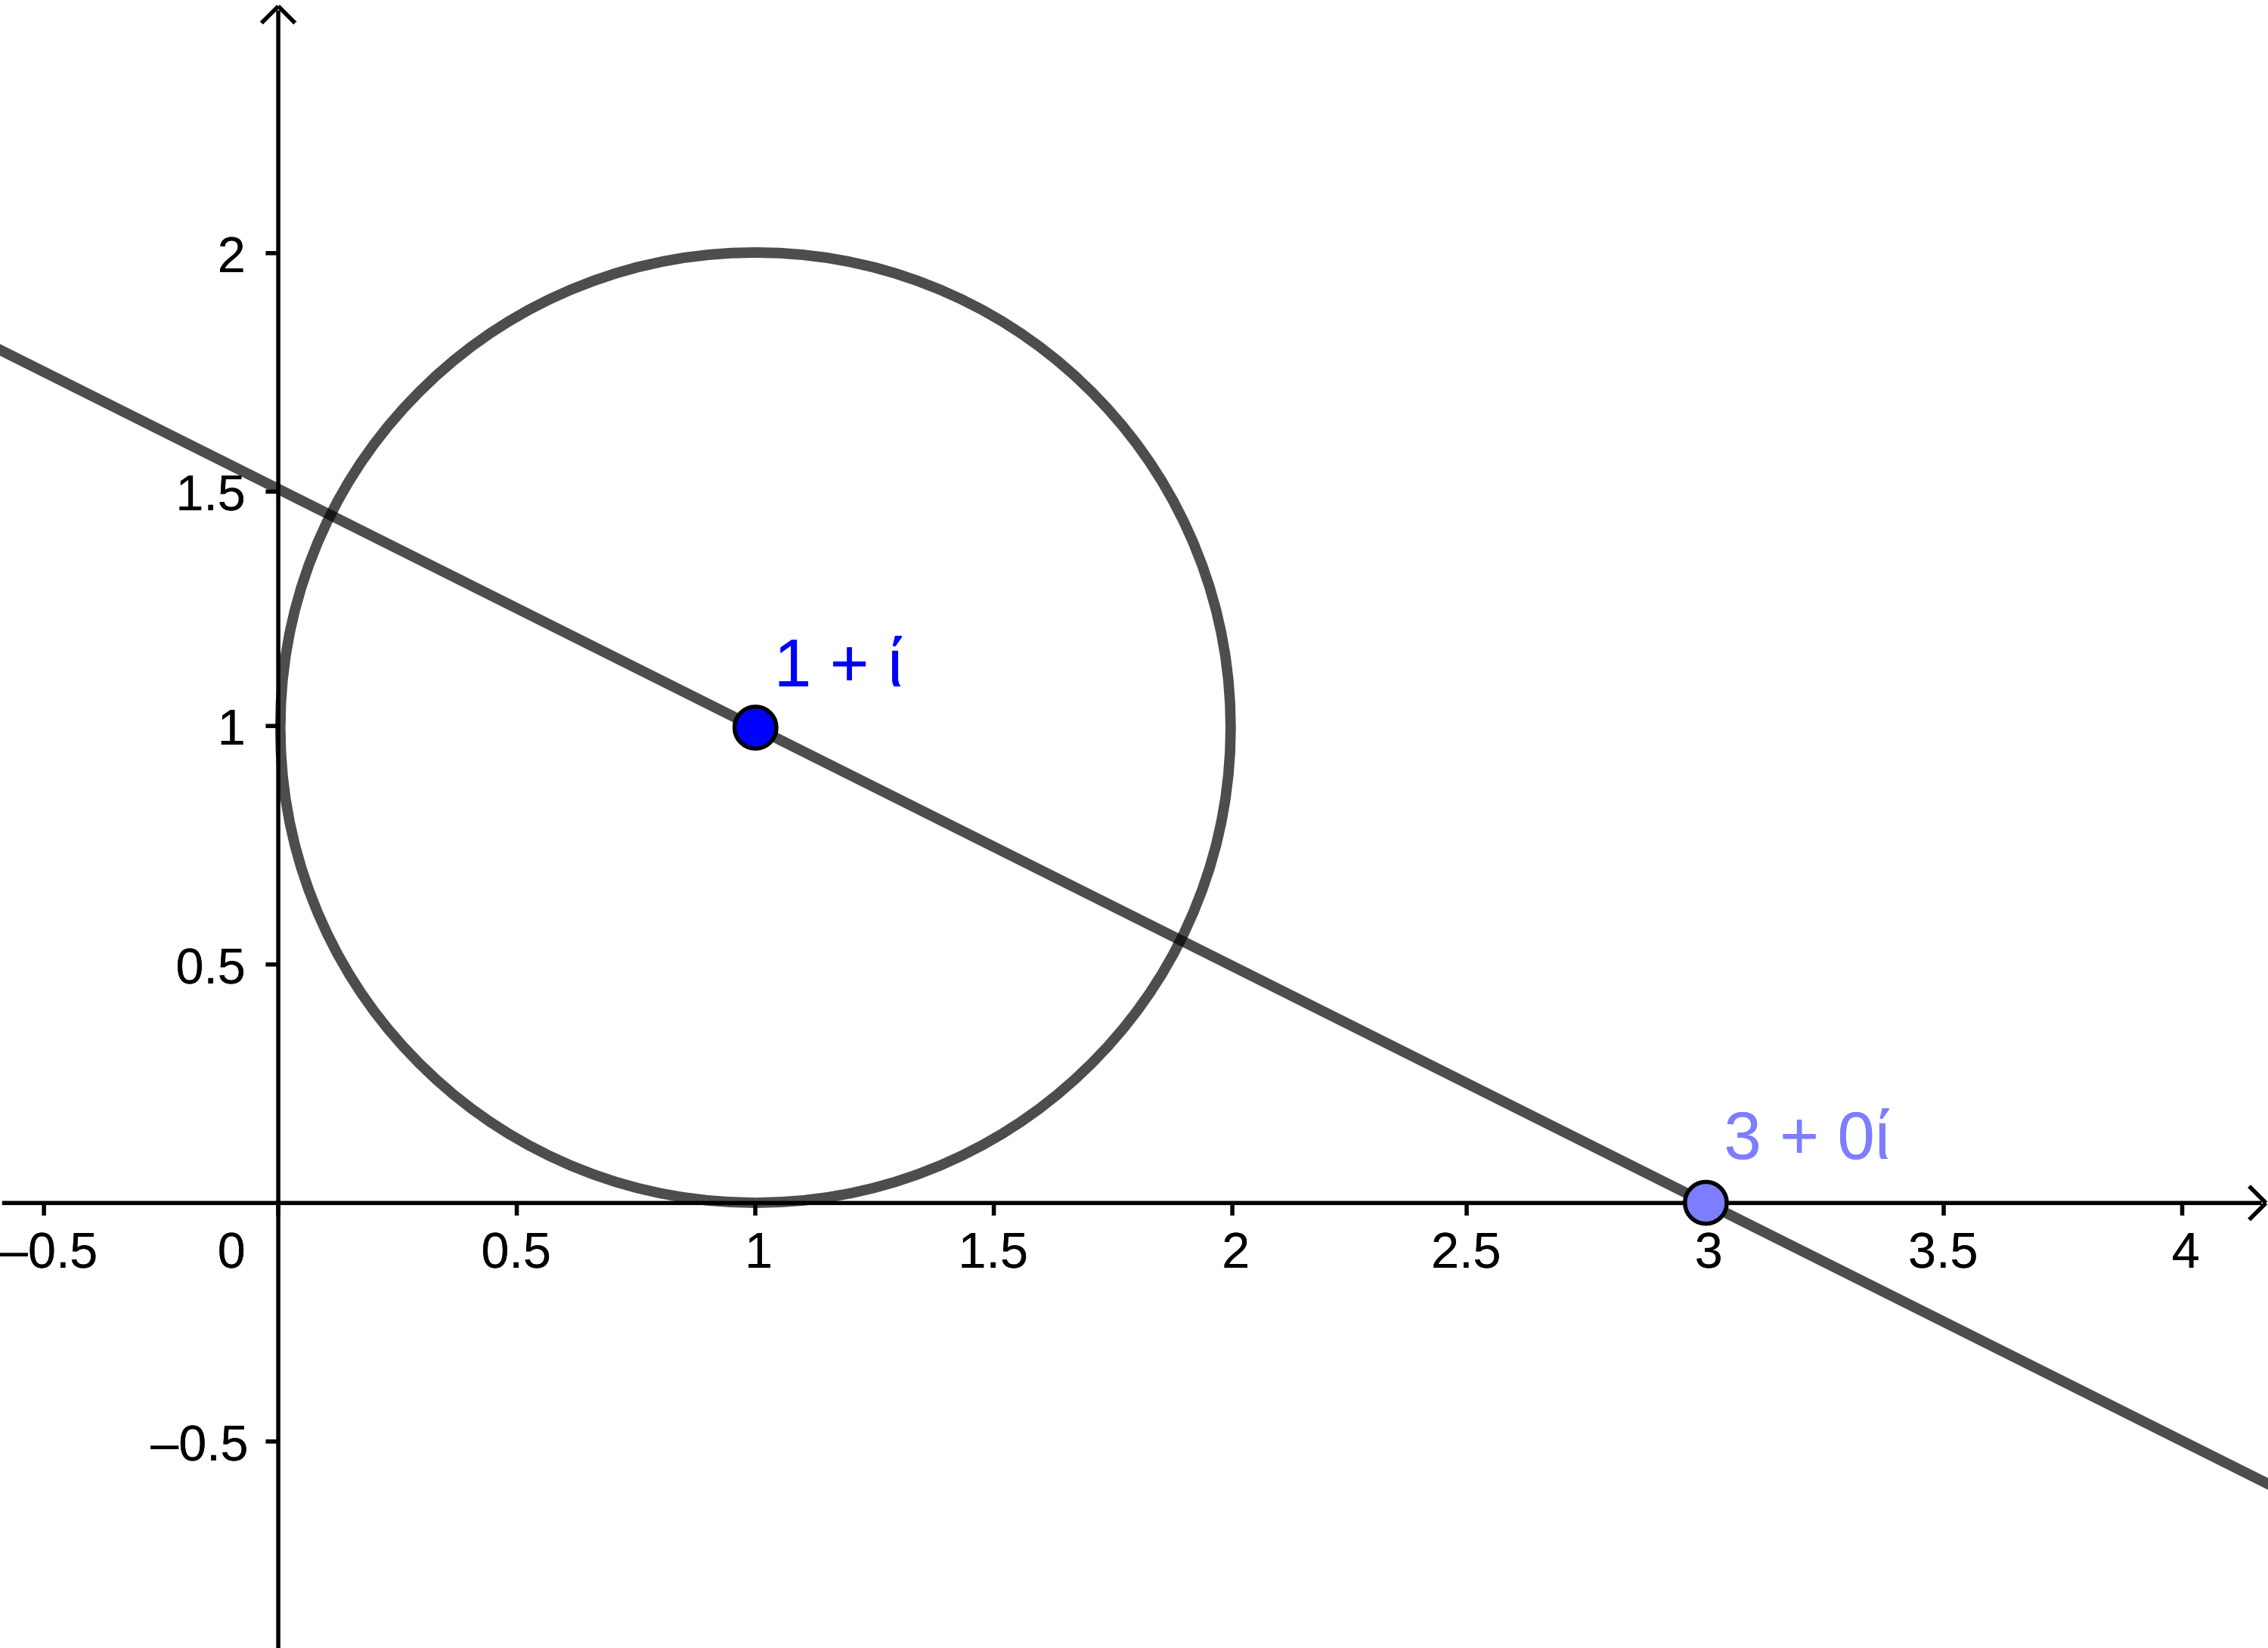
\includegraphics[width=0.5\textwidth]{q1_gg.png}
    \end{center}
   \end{figure}
   Alternatively, if we just draw the circle \(\abs{z - 1 - i} = 1\), and the
   line through \(i + 1\) and \(3\), then it is clear that the furthest point
   from \(3\) in D is the further intersection between the line and the circle,
   and likewise the closest point to \(3\) is the closer intersection. But the
   distance from \(3\) to \(1 + i\) is \(\sqrt 5\) and the radius of the circle
   is \(1\), so this gives the bounds \(\sqrt 5 - 1\) and \(\sqrt 5 + 1\).
   \item
    \begin{enumerate}[(i)]
     \item
      We have \(z = e^{i\theta} = \cos \theta + i \sin \theta\), for some
      \(\theta \in \intoc{-\pi, \pi}\). So then
      \begin{align*}
       1 + z &= 1 + \cos \theta + i \sin \theta \\
            &= 2 \cos^2 \tfrac 12 \theta
                  + i \cdot 2 \sin \tfrac 12 \theta \cos \tfrac 12 \theta \\
            &= 2 \cos \tfrac 12 \theta (\cos \tfrac 12 \theta
                                           + i \sin \tfrac 12 \theta) \\
            &= 2 \cos \tfrac 12 \theta
                       \exp\parens[\Big]{\frac{i\theta}2} \\
       \text{so}\quad \abs{1 + z} &= 2 \cos \tfrac 12 \theta \quad
                      \text{which is \(\ge 0\) as
                            \(\tfrac 12 \theta \in
                              \intoc{-\tfrac 12 \pi, \tfrac 12 \pi}\),} \\
                 \arg(1 + z) &= \tfrac 12 \theta \quad
                    \text{for \(\theta \ne \pi\)}
      \end{align*}
     \item
      Now instead take \(z = e^{i\theta} = \cos \theta + i \sin \theta\), for
      some \(\theta \in \intco{0, 2\pi}\). So then
      \begin{align*}
       1 - z &= 1 - \cos \theta - i \sin \theta \\
            &= 2 \sin^2 \tfrac 12 \theta
                  - i \cdot 2 \sin \tfrac 12 \theta \cos \tfrac 12 \theta \\
            &= 2 \sin \tfrac 12 \theta (\sin \tfrac 12 \theta
                                           - i \cos \tfrac 12 \theta) \\
            &= 2 \sin \tfrac 12 \theta (\cos \tfrac 12 (\theta - \pi)
                                           + i \sin \tfrac 12 (\theta - \pi)) \\
            &= 2 \sin \tfrac 12 \theta
                       \exp\parens[\Big]{\frac{i(\theta - \pi)}2} \\
       \text{so}\quad \abs{1 - z} &= 2 \sin \tfrac 12 \theta \quad
                         \text{which is \(\ge 0\) as
                         \(\tfrac 12 \theta \in \intco{0, \pi}\),} \\
                 \arg(1 - z) &= \tfrac 12 (\theta - \pi) \quad
                    \text{for \(\theta \ne 0\)}
      \end{align*}
    \end{enumerate}
    Geometrically, letting \(\theta\) be in \(\intoc{\pi, \pi}\) but starting by
    assuming \(\theta \ge 0\):
    \begin{enumerate}[(i)]
     \item
      Draw the circle with centre at \(1\), and radius \(1\) (the locus of
      \(1 + z\)). Then consider some value of \(1 + z\) on the circle. Draw a
      line from \(1 + z\) to \(1\), a line from \(1 + z\) to \(0\), and a line
      from \(0\) to \(1\) to form a triangle with two sides being radii of the
      circle.

      The exterior angle at \(1\) is \(\arg z = \theta\), so the
      interior angle is \(\pi - \theta\), and the triangle is isosceles so the
      two other angles must most be \(\frac 12 \theta\), implying
      \(\arg(1 + z)\) is indeed \(\frac 12 \theta\).

      If we also draw a line from \(1 + z\) to \(2\), forming a right angle
      subtended in the diameter of the circle on the real axis, then
      straightforward trigonometry shows that \(\abs{1 + z}\) is
      \(2 \cos \frac 12 \theta\), as the length of the hypotenuse is \(2\).

      If \(\theta < 0\) (ie \(\theta = -\theta'\) where \(\theta' > 0\)), the
      diagram just becomes inverted, so the modulus is
      \(2 \cos \frac 12 \theta' = 2 \cos \frac 12 \theta\) and the
      argument becomes \(-\frac 12 \theta' = \frac 12 \theta\), so this is fully
      consistent with the algebra.
     \item
      Now draw the triangle with vertices at \(0\), \(1 + z\), and \(1 - z\).
      One side is a diameter of the circle, so this is a right triangle. Then we
      can easily calculate that the (negative) angle between the real axis and
      the line to \(1 - z\) is \(\frac 12 (\pi - \theta)\), so indeed
      \(\arg(1 - z) = \frac 12 (\theta - \pi)\).

      We can also use Pythagoras in this triangle, as we know the length of the
      hypotenuse is \(\abs{1 + z - (1 - z)} = 2\). So
      \begin{alignat*}2
       && \abs{1 + z}^2 + \abs{1 - z}^2 &= 4 \\
       &\implies{}& \abs{1 - z} &= 2 \sqrt{1 - \cos^2 \tfrac 12 \theta} \\
       &&                       &= 2 \sin \tfrac 12 \theta \quad
                    \text{by the assumption that \(\theta \ge 0\)}
      \end{alignat*}
      \begin{figure}[H]
       \begin{center}
        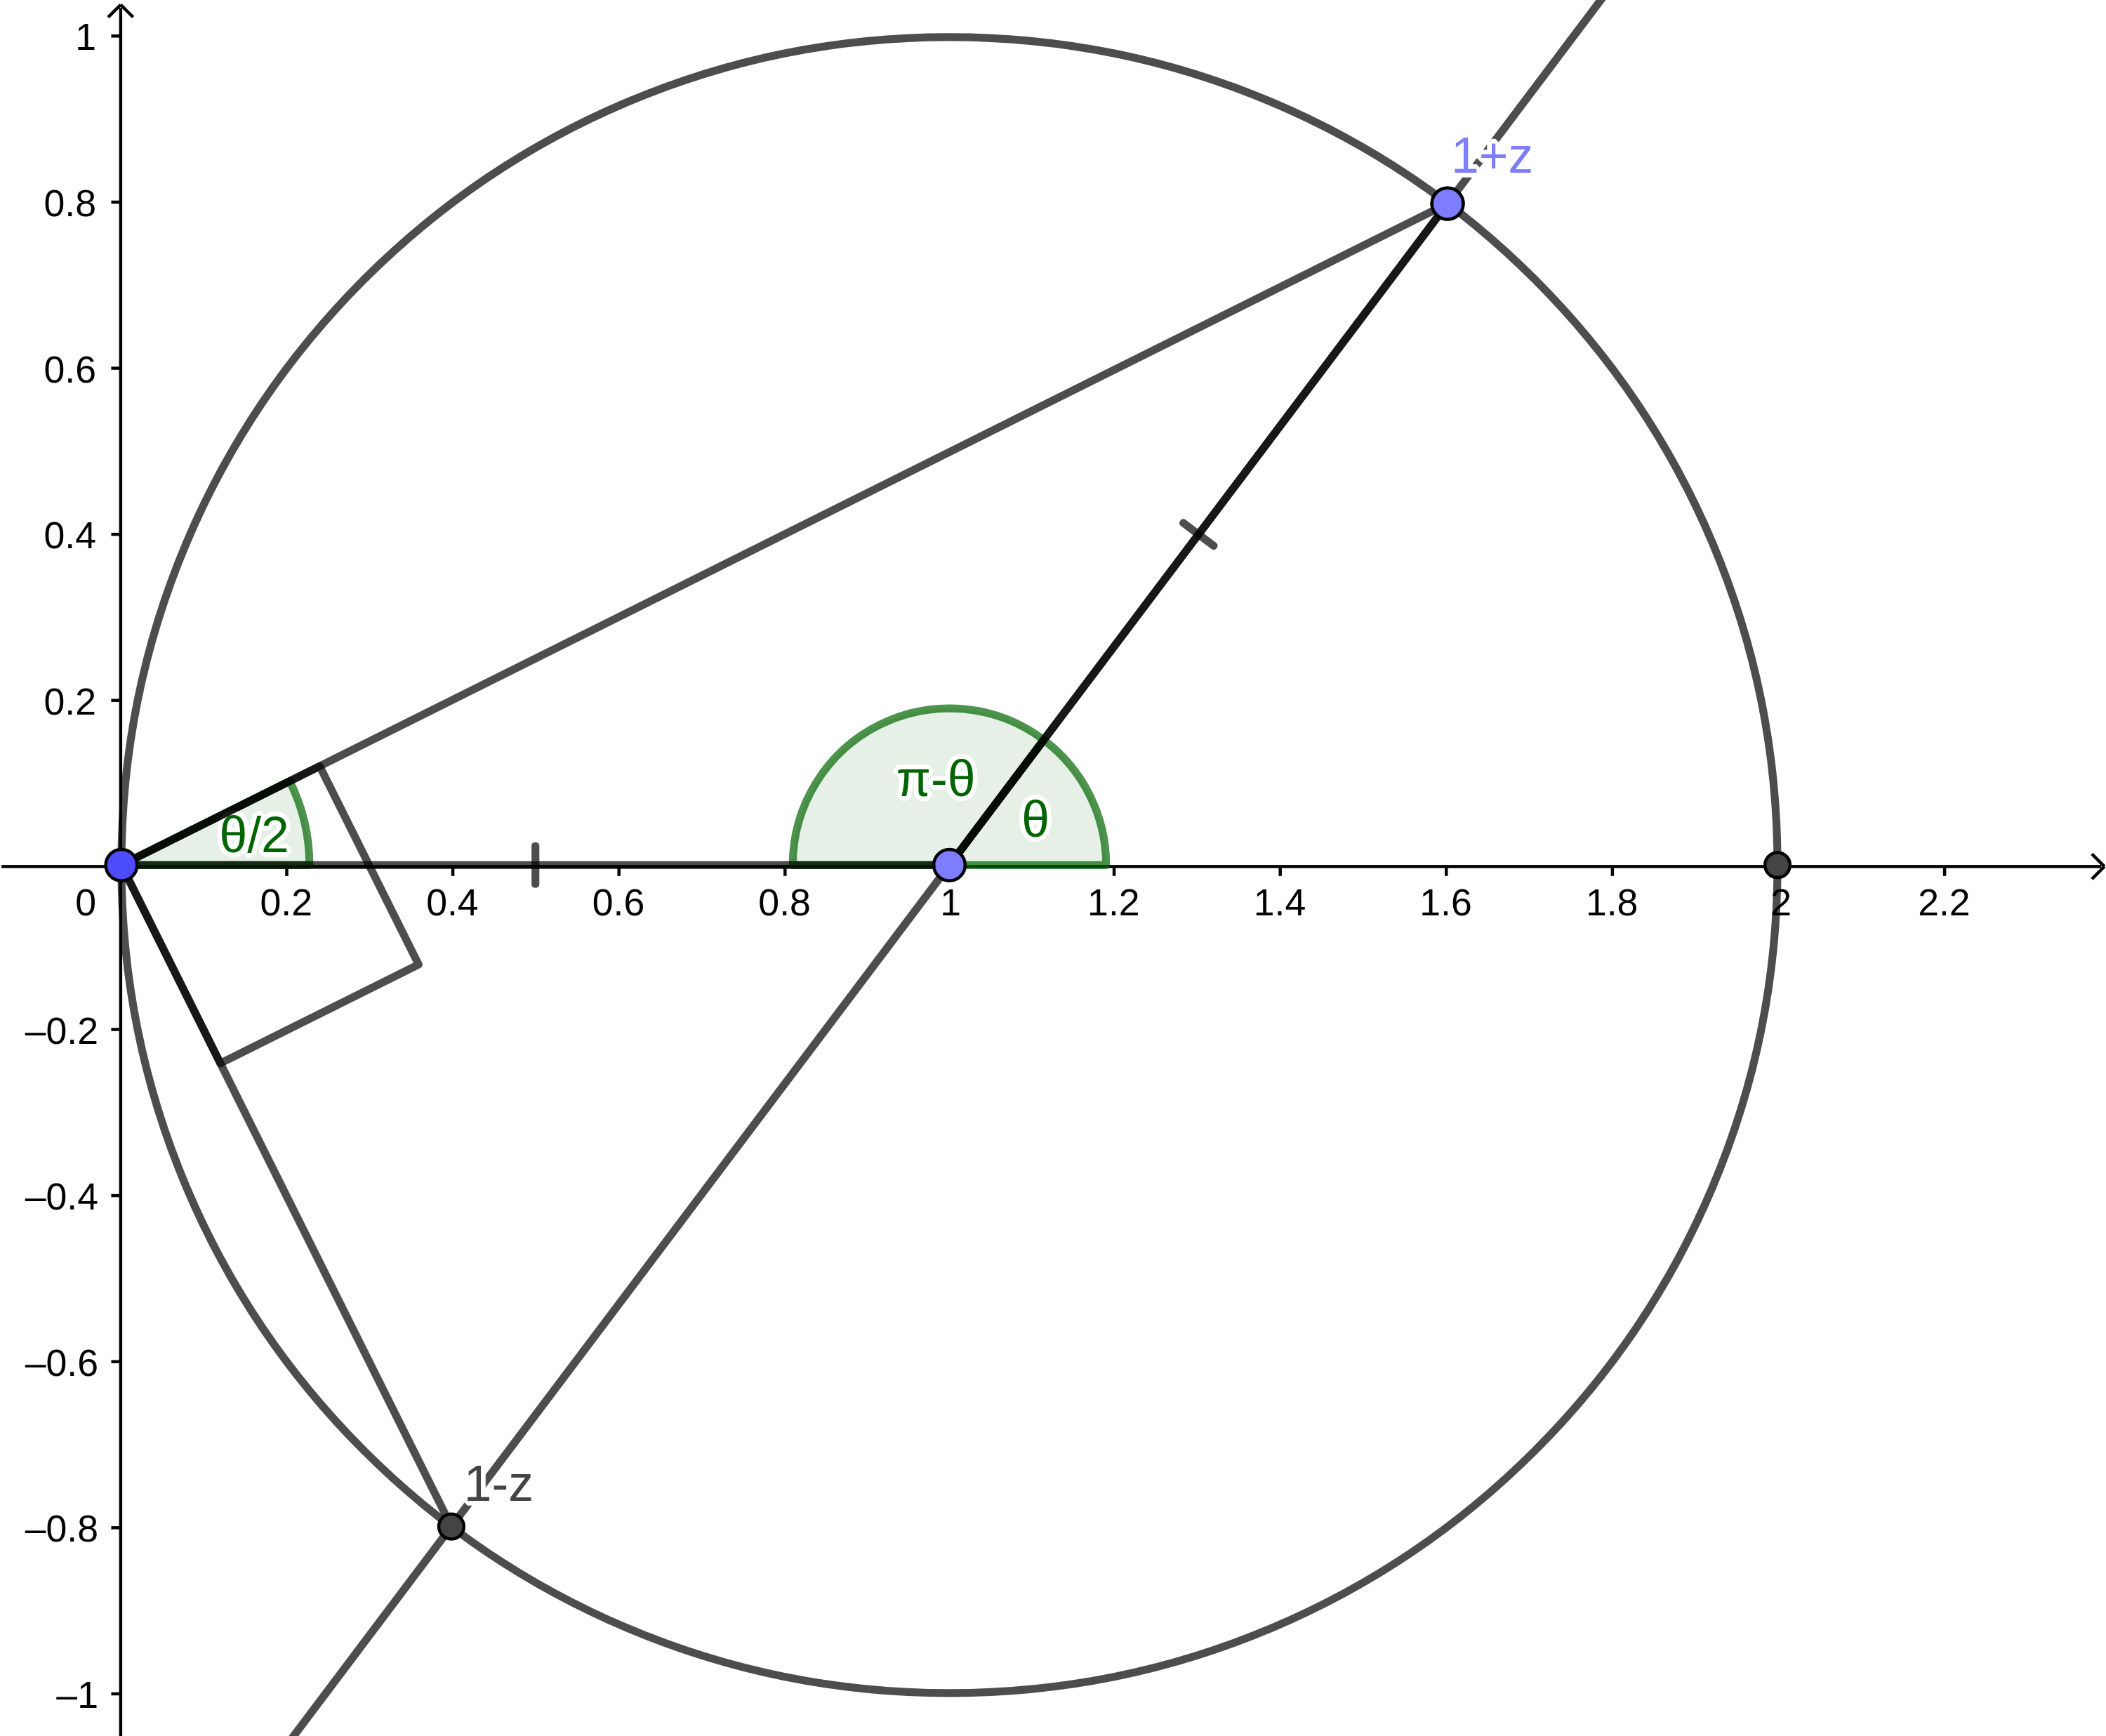
\includegraphics[width=0.5\textwidth]{q2_gg.png}
       \end{center}
      \end{figure}
      Now if the argument is \(< 0\) (ie \(\theta = -\theta'\) where
      \(\theta' > 0\)), the diagram is again reflected in the real axis.
      So the modulus is
      \(2\sin \frac 12 \theta' = -2\sin \frac 12 \theta
        = 2\sin \frac 12 (\theta + 2\pi)\).
      But now the argument must become
      \(-\frac 12 (\theta' - \pi) = \frac 12 (\theta + \pi)\).

      Both of these in fact correspond precisely to applying
      \(\theta \mapsto \theta + 2\pi\) when \(\theta < 0\) to switch to another
      branch of \(\arg\) to ``fix'' the range of the argument, so this is
      consistent with the algebra.
    \end{enumerate}
    Now we can rewrite
    \begin{align*}
     w^2 &= \frac{1 - z}{1 + z} \\
         &= \frac
             {2 \sin \tfrac 12 \theta \exp\parens[\Big]{\frac{i(\theta - \pi)}2}
             }
             {2 \cos \tfrac 12 \theta \exp\parens[\Big]{\frac{i\theta}2}} \quad
             \text{(nb neither of these used the range of
                   \(\theta\))} \\
         &= \tan \tfrac 12 \theta \exp\parens[\Big]{\frac{-i\pi}2} \\
         &= -i \tan \tfrac 12 \theta
    \end{align*}
    Now we consider two cases:
    \begin{alignat*}2
     \tan \tfrac 12 \theta &\ge 0 \implies&
      w &= \pm \sqrt{\tan \tfrac 12 \theta} \exp\parens[\Big]{\frac{-i\pi}4} \\
     && &= \pm \sqrt{\tan \tfrac 12 \theta} \,\frac{\sqrt 2}2 (1 - i) \\
     \tan \tfrac 12 \theta &< 0 \implies&
      w &= \pm \sqrt{-\tan \tfrac 12 \theta} \exp\parens[\Big]{\frac{i\pi}4} \\
     && &= \pm \sqrt{-\tan \tfrac 12 \theta} \,\frac{\sqrt 2}2 (1 + i)
    \end{alignat*}
    In both cases, \(\pm\sqrt{\abs{\tan \frac 12 \theta}}\) varies over all of
    \(\Reals\), so we get the two lines through the origin with gradients \(1\)
    and \(-1\), respectively.
   \item A point on the median through \(z_1\) has the form
    \begin{align*}
     w &= z_1 + \lambda (\tfrac 12 (0 + z_2) - z_1) \\
       &= z_1 + \lambda (\tfrac 12 z_2 - z_1)
    \end{align*}
    as addition of the complex number \(\frac 12 z_2 - z_1\) represents a
    translation from \(z_1\) in the direction of the midpoint of \(z_2\) and
    \(0\). Similarly, a point on the median through \(z_2\) has the form
    \begin{align*}
     w &= z_2 + \mu (\tfrac 12 (0 + z_1) - z_2) \\
       &= z_2 + \mu (\tfrac 12 z_1 - z_2)
    \end{align*}
    and a point on the median through 0 has the form
    \begin{align*}
     w &= 0 + \nu (\tfrac 12 (z_1 + z_2) - 0) \\
       &= \nu' (z_1 + z_2)
    \end{align*}
    Now we can equate the terms in \(z_1\) and \(z_2\), as they are linearly
    independent, to find the parameters at the intersection of the medians
    through \(z_1\) and \(z_2\):
    \begin{alignat*}2
     &z_1\colon\quad& 1 - \lambda &= \tfrac 12 \mu \\
     &z_2\colon\quad& 1 - \mu &= \tfrac 12 \lambda
    \end{alignat*}
    Then
    \(1 = \frac 12 \mu + \lambda = \frac 12 \lambda + \mu \implies
      \lambda = \mu\), and then
    \(1 - \lambda = \frac 12 \lambda \implies
      \mu = \lambda = \frac 23\). But then we are indeed on the median through
    zero, with \(\nu' = \frac 23\).
   \item For \(z \ne 1\),
    \begin{align*}
     I = \frac{z^5 - 1}{z - 1}
       &= \frac{(z - 1)(z^4 + z^3 + z^2 + z + 1)}{z - 1} \\
       &= z^4 + z^3 + z^2 + z + 1 \\
     \text{But also}\quad
     I &= \frac{(z - 1)(z - \omega)
                (z - \omega^2)(z - \omega^3)(z - \omega^4)}{z - 1} \\
       &= (z - \omega)(z - \omega^2)(z - \omega^3)(z - \omega^4) \\
       &= (z^2 - (\omega + \omega^4)z + \omega \omega^4)
          (z^2 - (\omega^2 + \omega^3)z + \omega^2\omega^3) \\
       &= (z^2 - (\omega + \omega^{-1})z + 1)
          (z^2 - (\omega^2 + \omega^{-2})z + 1) \\
       &= (z^2 - (2 \cos \tfrac 25 \pi)z + 1)
          (z^2 - (2 \cos \tfrac 45 \pi)z + 1) \\
       &\text{using \(\omega = e^{\frac 25 i\pi}\) and the exponentials
              definition of \(\cos\).}
    \end{align*}
    Expanding, the term in \(z^2\) has coefficient
    \(2 + 4\cos \frac 25 \pi \cos \frac 45 \pi\). But this is also equal to
    \(1\), from earlier. Then also using
    \(\cos \frac 25 \pi = \sin \frac 1{10} \pi\) and
    \(\cos \frac 45 \pi = - \cos \frac 15 \pi\), the result
    \(4 \cos \frac 15 \pi \sin \frac 1{10} \pi = 1\) follows.
   \item Using the definition of \(\sin z\) in complex exponentials:
    \begin{alignat*}3
     && \sin z &= 2 \\
     \iff{}&& \frac 1{2i}(e^{iz} - e^{-iz}) &= 2 \\
     \iff{}&& e^{2iz} - 4ie^{iz} - 1 &= 0 \\
     \iff{}&& e^{iz} &= \frac{4i \pm \sqrt{-16 + 4}}{2} \\
     &&              &= i(2 \pm \sqrt 3) \\
     &&              &= e^{\frac{i\pi}2 + \log(2 \pm \sqrt 3)} \\
     \iff{}&& iz &= i\pi(\tfrac 12 + 2n) + \log(2 \pm \sqrt 3),
                    \quad &&\text{with \(n \in \Integers\)} \\
     \iff{}&& z &= \pi(\tfrac 12 + 2n) - i\log(2 \pm \sqrt 3),
                    \quad &&\text{with \(n \in \Integers\)}
    \end{alignat*}
   \item
    \begin{enumerate}[(a)]
     \item Rewriting in terms of complex numbers,
      {\setlength{\mathindent}{-2cm}
      \begin{alignat*}2
       && \frac{\abs{\lseg{PA}}}{\abs{\lseg{PB}}} &= \lambda \\
       \iff{}&& \frac{\abs{z - a}}{\abs{z - b}} &= \lambda \\
       \iff{}&& \frac{\abs{z - a}^2}{\abs{z - b}^2} &= \lambda^2 \quad
        \text{as both sides are \(\ge 0\)} \\
       \iff{}&& \abs{z - a}^2 &= \lambda^2\abs{z - b}^2 \\
       \iff{}&& (z - a)(\conj{z - a}) &= \lambda^2(z - b)(\conj{z - b}) \\
       \iff{}&& (z - a)(\conj z - \conj a)
                 &= \lambda^2(z - b)(\conj z - \conj b) \\
       \iff{}&& 0 &= \lambda^2 z\conj z - \lambda^2 b \conj z
                     - \lambda^2 \conj b z
                     + \lambda^2 b \conj b - z \conj z + a \conj z
                     + \conj a z - a \conj a \\
       &&         &= (\lambda^2 - 1)z\conj z + (-\lambda^2 b + a)\conj z
                     + (-\lambda^2\conj b + \conj a)z
                     + \lambda^2 b\conj b - a\conj a \\
       &&         &= (\lambda^2 - 1)
                     \parens[\Big]{z - \frac{\lambda^2 b - a}{\lambda^2 - 1}}
                     \parens[\Big]{\conj z - \frac{\lambda^2 \conj b - \conj a}
                                                  {\lambda^2 - 1}} \\
       &&         &\phantom{={}}
                     - \frac{(\lambda^2 b - a)(\lambda^2 \conj b - \conj a)}
                            {\lambda^2 - 1}
                     + \lambda^2 b\conj b - a\conj a \quad
                                           \text{assuming \(\lambda \ne 1\)}\\
       \iff{}&&
                 (\lambda^2 - 1)^2
                     \abs[\Big]{z - \frac{\lambda^2 b - a}{\lambda^2 - 1}}^2
                  &=
                     (\lambda^2 b - a)(\lambda^2 \conj b - \conj a)
                     - (\lambda^2 - 1)(\lambda^2 b\conj b - a\conj a) \\
       &&         &= \lambda^4 b\conj b - \lambda^2 a\conj b
                     - \lambda^2 \conj ab + a\conj a
                     - (\lambda^4 b\conj b - \lambda^2 b\conj b
                     - \lambda^2 a\conj a + a\conj a) \\
       &&         &= \lambda^2(a\conj a - \conj a b - a\conj b + b\conj b) \\
       &&         &= \lambda^2(a - b)(\conj{a - b}) \\
       &&         &= \lambda^2\abs{a - b}^2 \\
       \iff{}&& \abs[\Big]{z - \frac{\lambda^2 b - a}{\lambda^2 - 1}}^2
                  &= \frac{\lambda^2}{(\lambda^2 - 1)^2}\abs{a - b}^2 \\
       \iff{}&& \abs[\Big]{z - \frac{\lambda^2 b - a}{\lambda^2 - 1}}
                  &= \frac{\lambda}{\abs{\lambda^2 - 1}}\abs{a - b}
      \end{alignat*}}
      Which is to say, if \(\lambda \ne 1\), \(C_\lambda\) corresponds precisely
      to the circle with centre \\ \((\lambda^2 b - a) / (\lambda^2 - 1)\) and
      radius \(\lambda \abs{a - b} / (\lambda^2 - 1)\).

      If \(\lambda = 1\), then \(C_\lambda\) is the locus of all \(\pnt P\)
      equidistant from \(\pnt A\) and \(\pnt B\), which is the perpendicular
      bisector of \(\pnt A\) and \(\pnt B\).
     \item
      We have \(a = -b\) and \(a, b \in \Reals\), so the perpendicular bisector
      of \(a\) and \(b\) is the imaginary axis. If
      \begin{equation*}
       S_\mu = \set[\Big]{z \in \Complex \mid
                          \abs{z - i\mu} = \textstyle\sqrt{p^2 + \mu^2}}
      \end{equation*}
      then \(S_\mu\) is the circle with centre \(i\mu\) (which is on the
      imaginary axis) and radius
      \(\sqrt{p^2 + \mu^2} = \sqrt{a^2 + \mu^2} = \sqrt{b^2 + \mu^2}\). Using
      Pythagoras' Theorem, the radius must then be the same as the distance from
      both \(a\) and \(b\) to \(i\mu\), the centre. So the circle passes through
      \(\pnt A\) and \(\pnt B\).

      Now \(C_\lambda\) is a circle with centre
      \(b(\lambda^2 + 1)/(\lambda^2 - 1) \in \Reals\), and radius
      \(\abs{2b}\abs{\lambda}/\abs{\lambda^2 - 1}\).

      Consider the triangle with vertices at the centres of \(C_\lambda\) and
      \(S_\mu\), and a vertex at the point where the tangent from the centre of
      \(C_\lambda\) meets \(S_\mu\).
      \begin{figure}[H]
       \begin{center}
        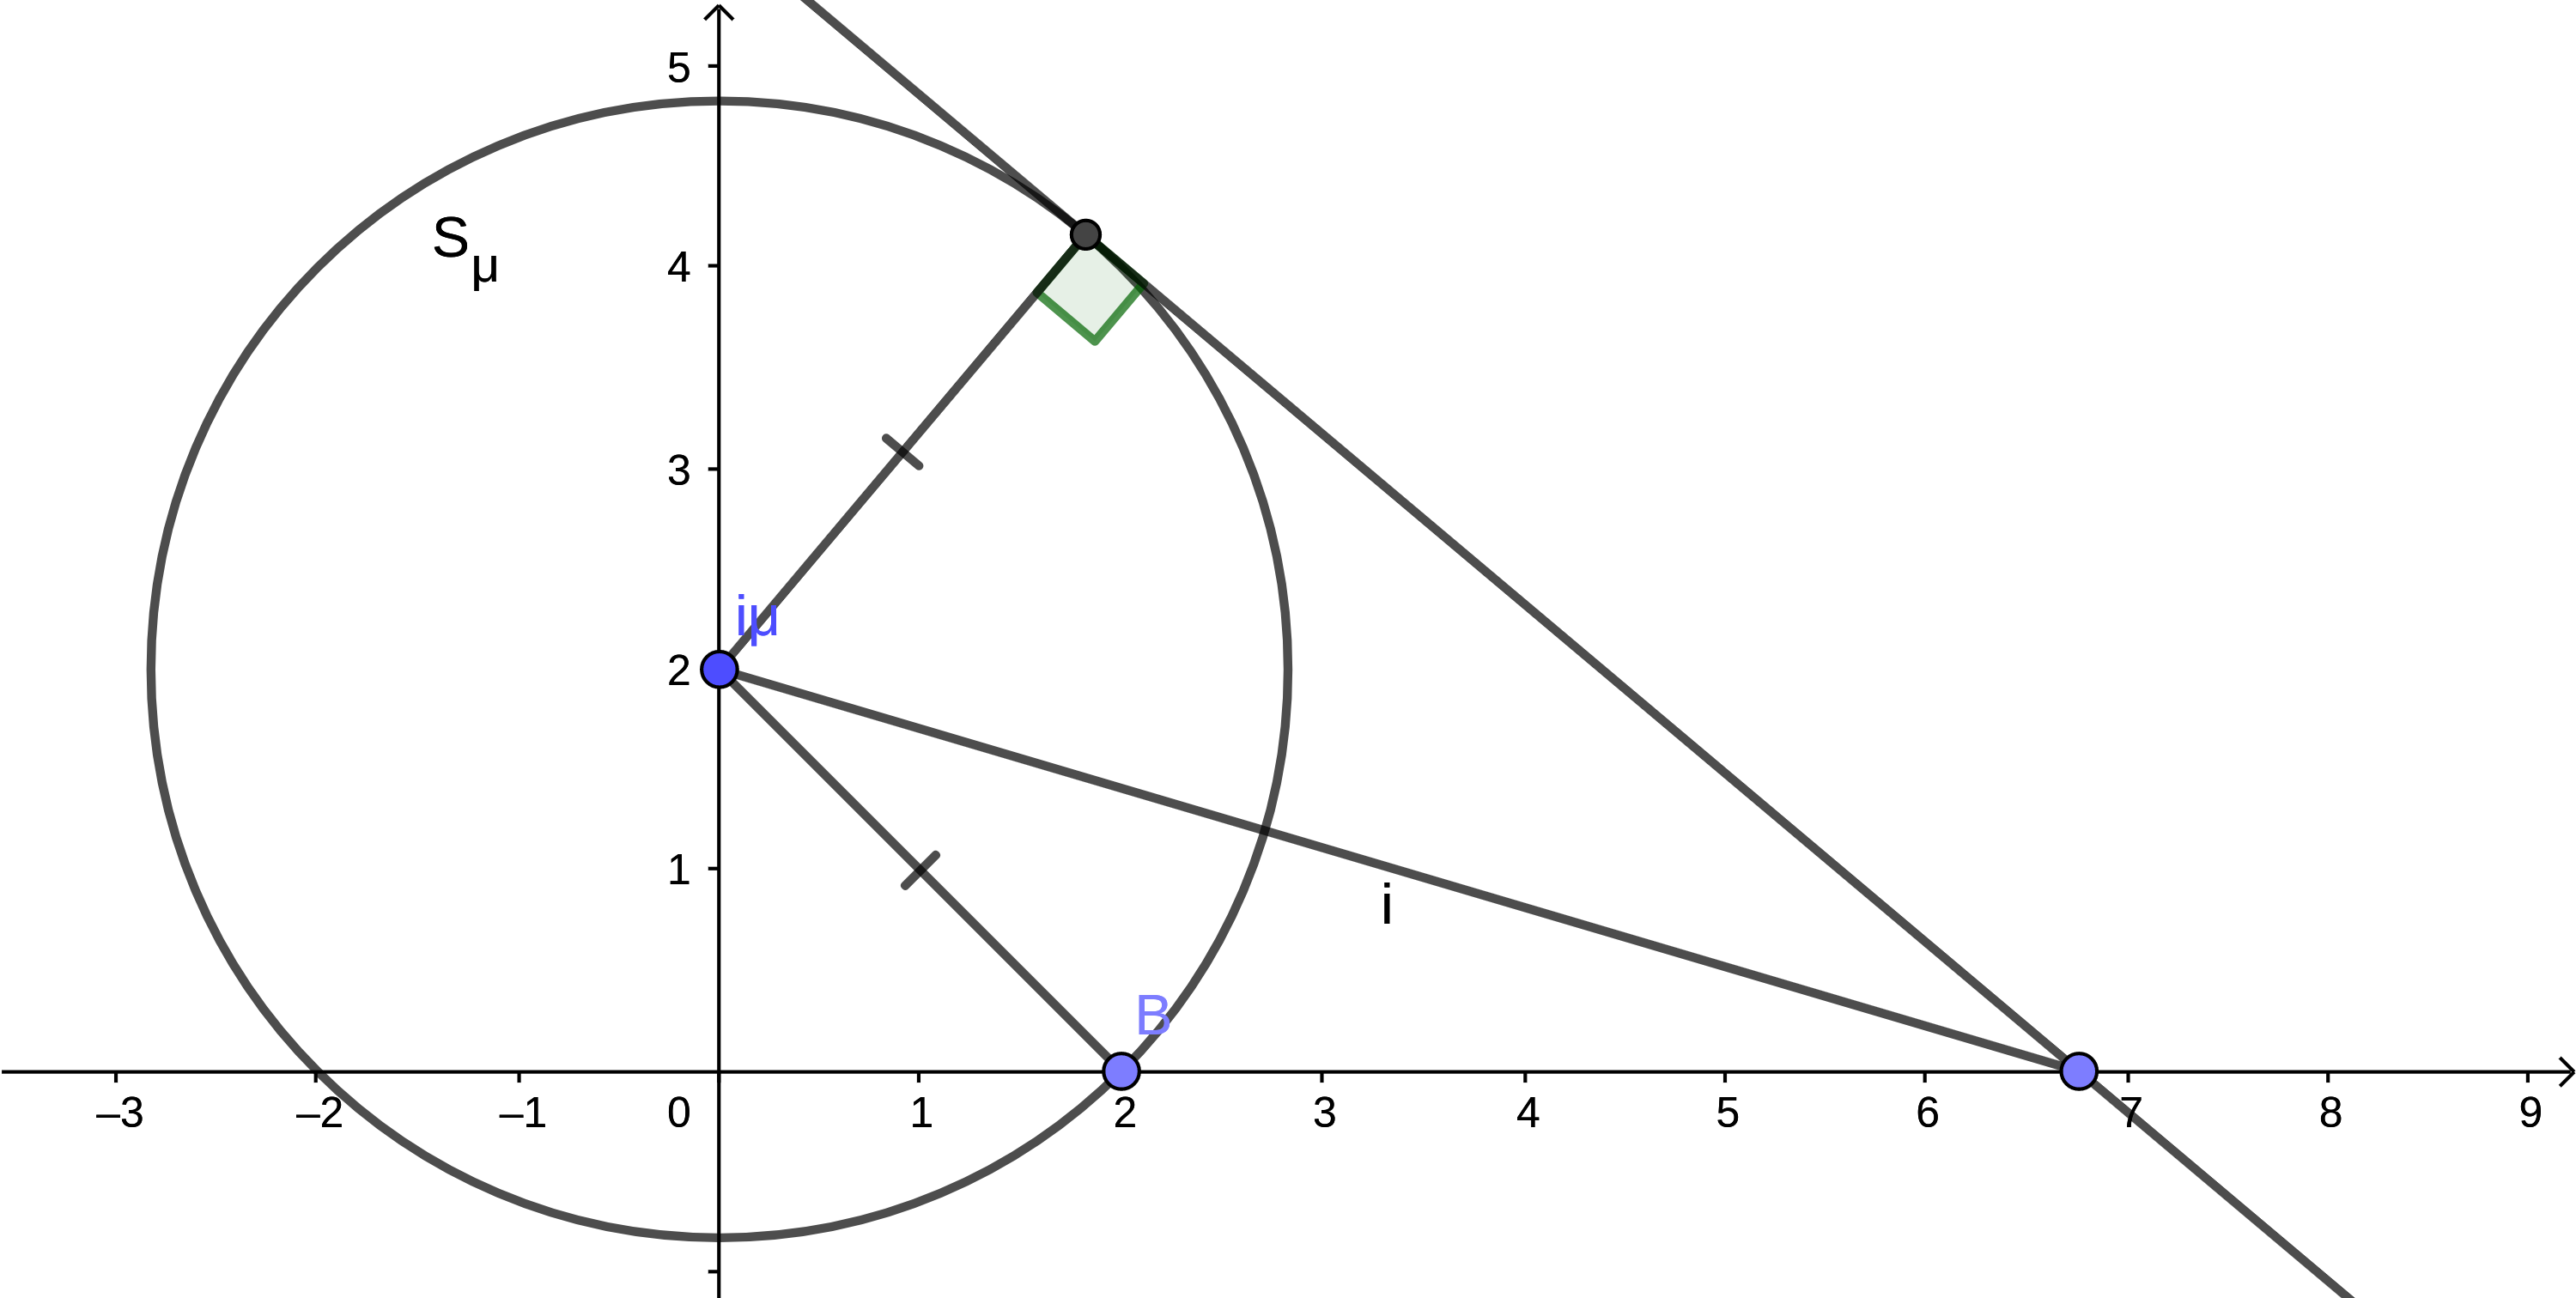
\includegraphics[width=0.5\textwidth]{q6_gg.png}
       \end{center}
      \end{figure}
      This triangle has a right angle by construction, as tangents are
      perpendicular to radii. So then we calculate the distance \(d\) that the
      centre of \(C_\lambda\) is along the tangent from \(S_\mu\), using
      Pythagoras:
      \begin{align*}
       d^2 &= b^2 \parens[\Big]{\frac{\lambda^2 + 1}{\lambda^2 - 1}}^2
             + \mu^2 - (b^2 + \mu^2) \\
           &= b^2\parens[\bigg]{
                  \parens[\Big]{\frac{\lambda^2 + 1}{\lambda^2 - 1}}^2
                  - 1
                 } \\
           &= b^2 \cdot
                \frac{2\lambda^2}{\lambda^2 - 1} \cdot
                \frac{2}{\lambda^2 - 1} \\
           &= \parens[\Big]{\frac{2b\lambda}{\lambda^2 - 1}}^2
      \end{align*}
      So in fact the tangent is exactly a radius of \(C_\lambda\), and
      \(C_\lambda\) and \(S_\mu\) must intersect orthogonally (the other point
      of intersection has the same angle of intersection, by symmetry).
    \end{enumerate}
   \item
    Following the hint, let \(\lseg{AD}\) and \(\lseg{BE}\) be altitudes,
    meeting at \(H\). Then we have: \(\veca{AH} \vecdot \veca{BC} = 0\) and
    \(\veca{BH} \vecdot \veca{AC} = 0\)
    by definition of altitudes, and we want \(\veca{CH} \vecdot \veca{AB} = 0\).
    Proceed by substituting other paths through the triangle:
    \begin{align*}
     \veca{CH} \vecdot \veca{AB}
      &= (\veca{CA} + \veca{AH}) \vecdot \veca{AB} \\
      &= \veca{CA} \vecdot \veca{AB} + \veca{AH} \vecdot \veca{AB} \\
      &= \veca{CA} \vecdot (\veca{AH} + \veca{HB})
         + \veca{AH} \vecdot \veca{AB} \\
      &= \veca{CA} \vecdot \veca{AH}
         + \underbrace{\veca{CA} \vecdot \veca{HB}}_{= -0}
         + \veca{AH} \vecdot \veca{AB} \\
      &= \veca{CA} \vecdot \veca{AH} + \veca{AH} \vecdot \veca{AB} \\
      &= \veca{AH} \vecdot (\veca{CA} + \veca{AB}) \\
      &= \veca{AH} \vecdot \veca{CB}, \quad \text{by contracting} \\
      &= 0
    \end{align*}
    so \(\lseg{CH}\) is perpendicular to \(\lseg{AB}\), ie the altitude through
    \(\pnt C\) also passes through the point of intersection of the altitudes
    from \(\pnt A\) and \(\pnt B\), so all three altitudes are concurrent.
   \item
    Applying \(\vec v \mapsto \vec v \vecdot \vec v\) to both sides,
    \begin{alignat*}2
     &&  \vec x + \vec y (\vec x \vecdot \vec y) &= \vec a \\
     \implies{}&&
         (\vec x + \vec y (\vec x \vecdot \vec y)) \vecdot
         (\vec x + \vec y (\vec x \vecdot \vec y)) &=
         \vec a \vecdot \vec a \\
     \implies{}&& \abs{\vec x}^2
                  + 2(\vec x \vecdot \vec y)(\vec x \vecdot \vec y)
                  + \abs{\vec y}^2(\vec x \vecdot \vec y)^2 &=
                  \abs{\vec a}^2 \\
     \implies{}&& (\vec x \vecdot \vec y)^2 (2 + \abs{\vec y}^2) &=
                  \abs{\vec a}^2 - \abs{\vec x}^2 \\
     \implies{}&& (\vec x \vecdot \vec y)^2 &=
                  \frac{\abs{\vec a}^2 - \abs{\vec x}^2}{2 + \abs{\vec y}^2}
    \end{alignat*}
    But we have the Cauchy-Shwarz inequality:
    \(\vec x \vecdot \vec y \le \abs{\vec x}\abs{\vec y}\), so
    \begin{alignat*}2
     && \frac{\abs{\vec a}^2 - \abs{\vec x}^2}{2 + \abs{\vec y}^2} &\le
        \abs{\vec x}^2\abs{\vec y}^2 \\
     \implies{}&& \abs{\vec a}^2 - \abs{\vec x}^2 &\le
        \abs{\vec x}^2\abs{\vec y}^2(2 + \abs{\vec y}^2) \quad
        \text{as \(2 + \abs{\vec y}^2 \ge 2 > 0\)} \\
     \implies{}&& \abs{\vec a}^2 &\le
        \abs{\vec x}^2(1 + \abs{\vec y}^2(2 + \abs{\vec y}^2)) \\
     &&        &= \abs{\vec x}^2(1 + \abs{\vec y}^2)^2
    \end{alignat*}
    So we have \(\abs{\vec a} \le \abs{\vec x}(1 + \abs{\vec y}^2)\).
    But also from earlier
    \(\abs{\vec a}^2 = \abs{\vec x}^2 + 2(\vec x \vecdot \vec y)^2
                       + \abs{\vec y}^2(\vec x \vecdot \vec y)^2
                     \ge \abs{\vec x}^2\)
    so \(\abs{\vec a} \ge \abs{\vec x}\).

    If \(\abs{\vec a} = \abs{\vec x}\), then \(\vec x \vecdot \vec y = 0\), from
    the equation for \((\vec x \vecdot \vec y)^2\). But then from the original
    relation, we have \(\vec x = \vec a\). So the condition here is
    \(\vec x = \vec a\) and \(\vec x\) perpendicular to \(\vec y\).

    If \(\abs{\vec a} = \abs{\vec x}(1 + \abs{\vec y}^2)\), then we need
    \(\vec x = \lambda \vec y\) or \(\vec y = \vec 0\) or \(\vec x = \vec 0\)
    (some \(0 \ne \lambda \in \Reals\)), as this
    could only be an equality if Cauchy-Shwarz is.
    \begin{alignat*}2
     \text{
      If \(\vec x = \lambda \vec y\)}\colon
          && \quad \lambda \vec y + \vec y (\lambda \abs{\vec y}^2) &= \vec a \\
     \implies{}&& \vec y &= \frac 1{\lambda(1 + \abs{\vec y}^2)}\,\vec a \\
     && \text{and then} \quad \vec x &=
             \frac 1{1 + \abs{\vec y}^2}\,\vec a \\
     \intertext{
      So we have \(\vec x\), \(\vec y\) parallel to \(\vec a\), and determined
      by the choice of \(\abs{\vec y}\) and the value of \(\lambda\).}
     \text{
      If \(\vec x\) or \(\vec y\) is \(\vec 0\)}\colon
     && \quad \vec x + 0\vec y &= \vec a
    \end{alignat*}
    so either:
    \begin{itemize}
     \item \(\vec x = \vec a = \vec 0\) and \(\vec y\) is an arbitrary vector
     \item \(\vec y = \vec 0\) and \(\vec x = \vec a\) is an arbitrary vector
    \end{itemize}
   \item
    \begin{enumerate}
     \item
      Using
      \(\veca{AB} = -\veca{CA} - \veca{BC} \implies \vec u = -\vec v - \vec w\)
      and
      \(\veca{BC} = -\veca{AB} - \veca{CA} \implies \vec v = -\vec u - \vec w\)
      as well as the anticommutativity of \(\veccross\) and the distributivity
      of \(\veccross\) over \(+\) and the fact that
      \(\vec x \veccross \vec x = \vec 0\),
      \begin{align*}
       \vec u \veccross \vec v &= (-\vec v - \vec w) \veccross \vec v \\
                               &= \vec 0 - \vec w \veccross \vec v \\
                               &= \vec v \veccross \vec w \\
                               &= (-\vec u - \vec w) \veccross \vec w \\
                               &= -\vec u \veccross \vec w - \vec 0 \\
                               &= \vec w \veccross \vec u
      \end{align*}
      Taking magnitudes, and labeling the angles and sides as in the sine rule,
      we then have
      \begin{alignat*}3
       && \abs{\vec u}\abs{\vec v}\sin B &={}&
          \abs{\vec v}\abs{\vec w}\sin C &=
          \abs{\vec w}\abs{\vec u}\sin A \\
       \implies{}&&
          ca\sin B &={}&
          ab\sin C &=
          bc\sin A \\
       \implies{}&&
          \frac{\sin B}b &={}&
          \frac{\sin C}c &=
          \frac{\sin A}a
      \end{alignat*}
     \item
      Using distributivity, anticommutativity, and
      \(\vec p \veccross \vec p = \vec 0\),
      \begin{align*}
       \vec 0 &= \vec 0 + \vec p \veccross \vec q - \vec p \veccross \vec q \\
              &= \vec p \veccross \vec p + \vec p \veccross \vec q
                 - \vec r \veccross \vec p \\
              &= \vec p \veccross \vec p + \vec p \veccross \vec q
                 + \vec p \veccross \vec r \\
              &= \vec p \veccross (\vec p + \vec q + \vec r) \\
       \intertext{But by symmetry/the same argument,}
       \vec 0 &= \vec q \veccross (\vec p + \vec q + \vec r)
      \end{align*}
      So if \(\vec p + \vec q + \vec r\) was non-null, then it would be parallel
      to both \(\vec p\) and \(\vec q\). But we have
      \(\vec p \veccross \vec q \ne \vec 0 \implies
        \vec p \nparallel \vec q\), so we can conclude
      \(\vec p + \vec q + \vec r = \vec 0\).
    \end{enumerate}
   \item
    \begin{enumerate}
     \item
      If \(\vec a = \vec b\), then \(\vec r = \vec a = \vec b\), which is
      obviously symmetric, and mostly uninteresting. If not,
      \begin{align*}
       \vec r &= (1 - \lambda)\vec a + \lambda \vec b \\
              &= \vec a + \lambda(\vec b - \vec a)
      \end{align*}
      which is to say that \(\vec r\) lies on the line through \(\pnt A\) with
      direction vector \(\vec b - \vec a\), also known as the line through
      \(\pnt A\) and \(\pnt B\). This can also be written
      \begin{alignat*}2
       && (\vec r - \vec a) \veccross (\vec b - \vec a) &= \vec 0 \\
       \iff{}&& \vec r \veccross \vec b - \vec r \veccross \vec a
                - \vec a \veccross \vec b &= \vec 0 \\
      \intertext{Exchanging \(\vec a\) and \(\vec b\), we then get}
       && \vec r \veccross \vec a - \vec r \veccross \vec b
                - \vec b \veccross \vec a &= \vec 0 \\
       \iff{}&& \vec r \veccross \vec b - \vec r \veccross \vec a
                + \vec b \veccross \vec a &= \vec 0 \\
       \iff{}&& \vec r \veccross \vec b - \vec r \veccross \vec a
                - \vec a \veccross \vec b &= \vec 0
      \end{alignat*}
      so, as expected, the set of points on the line through \(\pnt A\) and
      \(\pnt B\) is independent of the ordering of \(\pnt A\) and \(\pnt B\).
     \item
      If \(\pnt A\), \(\pnt B\), \(\pnt C\) are all the same point, then
      \(\vec r = \vec a = \vec b = \vec c\) (again, symmetric). If they are not
      the same point but collinear, then this reduces to a line (see previous
      case, taking any two distinct points
      from \(\set{\pnt A, \pnt B, \pnt C}\)). If not,
      \begin{align*}
       \vec r &= (1 - \lambda - \mu)\vec a + \lambda \vec b + \mu \vec c \\
              &= \vec a + \lambda(\vec b - \vec a) + \mu (\vec c - \vec a)
      \end{align*}
      which is to say that \(\vec r\) lies on the plane through \(\pnt A\) such
      that the vectors \(\vec b - \vec a\) and \(\vec c - \vec a\) are along the
      plane, also known as the plane through \(\pnt A\), \(\pnt B\), and
      \(\pnt C\).

      They aren't collinear, so we can construct a normal vector to
      the plane: \((\vec b - \vec a) \veccross (\vec c - \vec a) \ne \vec 0\).
      Then we can write the plane as
      \begin{alignat*}2
       && \vec r \vecdot ((\vec b - \vec a) \veccross (\vec c - \vec a)) &= 0 \\
       \iff{}&& \vec r \vecdot
                (\vec b \veccross \vec c - \vec b \veccross \vec a
                 - \vec a \veccross \vec c) &= 0 \\
       \intertext{
        Exchanging \(\vec a\), \(\vec b\):}
       && \vec r \vecdot
                (\vec a \veccross \vec c - \vec a \veccross \vec b
                 - \vec b \veccross \vec c) &= 0 \\
       \iff{}&& \vec r \vecdot
                (\vec a \veccross \vec c + \vec b \veccross \vec a
                 - \vec b \veccross \vec c) &= 0 \\
       \iff{}&& \vec r \vecdot
                (\vec b \veccross \vec c - \vec b \veccross \vec a
                 - \vec a \veccross \vec c) &= 0 \\
       \intertext{
        Exchanging \(\vec b\), \(\vec c\):}
       && \vec r \vecdot
                (\vec c \veccross \vec b - \vec c \veccross \vec a
                 - \vec a \veccross \vec b) &= 0 \\
       \iff{}&& \vec r \vecdot
                (-\vec b \veccross \vec c + \vec a \veccross \vec c
                 + \vec b \veccross \vec a) &= 0 \\
       \iff{}&& \vec r \vecdot
                (\vec b \veccross \vec c - \vec b \veccross \vec a
                 - \vec a \veccross \vec c) &= 0
      \end{alignat*}
      These two transpositions generate all permutations
      \footnote{See ``BubbleSort''} of
      \(\set{\vec a, \vec b, \vec c}\), so we are done, and indeed the plane
      does not change upon reordering \(\pnt A\), \(\pnt B\), \(\pnt C\).
    \end{enumerate}
   \item
    \begin{enumerate}
     \item
      \begin{enumerate}[(i)]
       \item
        Using
        \([\vec a \veccross \vec b, \vec c, \vec d] =
          [\vec c, \vec d, \vec a \veccross \vec b]\),
        \begin{align*}
         (\vec a \veccross \vec b) \vecdot (\vec c \veccross \vec d) &=
          \vec c \vecdot (\vec d \veccross (\vec a \veccross \vec b)) \\
          &= \vec c \vecdot ((\vec d \vecdot \vec b)\vec a
                             - (\vec d \vecdot \vec a)\vec b) \\
          &= (\vec d \vecdot \vec b)(\vec a \vecdot \vec c)
             - (\vec d \vecdot \vec a)(\vec b \vecdot \vec c) \\
          &= (\vec a \vecdot \vec c)(\vec b \vecdot \vec d)
             - (\vec a \vecdot \vec d)(\vec b \vecdot \vec c)
        \end{align*}
       \item
        Doing lots of algebra and commuting the dot products, everything
        cancels:
        \begin{align*}
         &\phantom{={}} \vec a \veccross (\vec b \veccross \vec c) +
            \vec b \veccross (\vec c \veccross \vec a) +
            \vec c \veccross (\vec a \veccross \vec b) \\
         &= (\vec a \vecdot \vec c)\vec b - (\vec a \vecdot \vec b)\vec c
           + (\vec b \vecdot \vec a)\vec c - (\vec b \vecdot \vec c)\vec a
           + (\vec c \vecdot \vec b)\vec a - (\vec c \vecdot \vec a)\vec b \\
         &= (\vec a \vecdot \vec c)\vec b - (\vec a \vecdot \vec b)\vec c
           + (\vec a \vecdot \vec b)\vec c - (\vec b \vecdot \vec c)\vec a
           + (\vec c \vecdot \vec b)\vec a - (\vec a \vecdot \vec c)\vec b \\
         &= \vec 0
        \end{align*}
      \end{enumerate}
      Letting \(\vec c = \vec a\) and \(\vec d = \vec b\) in (i), and letting
      \(\theta\) be the angle between \(\vec a\) and \(\vec b\),
      \begin{alignat*}2
       && (\vec a \veccross \vec b) \vecdot (\vec a \veccross \vec b)
        &= (\vec a \vecdot \vec a)(\vec b \vecdot \vec b)
           - (\vec a \vecdot \vec b)(\vec a \vecdot \vec b) \\
       \implies{}&&
        \abs{\vec a \veccross \vec b}^2
        &= \abs{\vec a}^2 \abs{\vec b}^2
           - (\abs{\vec a}\abs{\vec b}\cos \theta)^2 \\
       \implies{}&&
        (\abs{\vec a} \abs{\vec b} \sin \theta)^2
        &= \abs{\vec a}^2 \abs{\vec b}^2
           - (\abs{\vec a}\abs{\vec b}\cos \theta)^2 \\
       \implies{}&&
        0 &= \abs{\vec a}^2 \abs{\vec b}^2(1 - \cos^2 \theta - \sin^2 \theta)
      \end{alignat*}
      So by finding non-null \(\vec a\) and \(\vec b\) at an angle of
      \(\theta\), we have shown the standard Pythagorean identity for
      \(\theta\): \(\sin^2 \theta + \cos^2 \theta = 1\).

      Using the anticommutative property of \(\veccross\),
      \begin{alignat*}2
       && (\vec a \veccross \vec b) \veccross (\vec c \veccross \vec d) &=
          - (\vec c \veccross \vec d) \veccross (\vec b \veccross \vec a) \\
       \implies{}&&
          ((\vec a \veccross \vec b) \vecdot \vec d)\vec c
          - ((\vec a \veccross \vec b) \vecdot \vec c)\vec d &=
          -( ((\vec c \veccross \vec d) \vecdot \vec b)\vec a
             - ((\vec c \veccross \vec d) \vecdot \vec a)\vec b)
      \end{alignat*}
      So, rearranging,
      \begin{equation*}
       ((\vec c \veccross \vec d) \vecdot \vec b)\vec a
       - ((\vec c \veccross \vec d) \vecdot \vec a)\vec b
       + ((\vec a \veccross \vec b) \vecdot \vec d)\vec c
       - ((\vec a \veccross \vec b) \vecdot \vec c)\vec d = \vec 0
      \end{equation*}
      If this is not the trivial linear combination, then the whole set is
      linearly dependent.

      If this is the trivial linear combination, then each of the scalar triple
      products of any three of \(\vec a\), \(\vec b\), \(\vec c\), \(\vec d\) is
      0, so, for instance, \(\set{\vec a, \vec b, \vec c}\) is linearly
      dependent, and the whole set must also be linearly dependent.
     \item Expanding,
      \begin{align*}
       [\vec a \veccross \vec b,
        \vec b \veccross \vec c,
        \vec c \veccross \vec a] &=
         (\vec a \veccross \vec b) \vecdot
         ((\vec b \veccross \vec c) \veccross (\vec c \veccross \vec a)) \\
        &= (\vec a \veccross \vec b)  \vecdot
           [((\vec b \veccross \vec c) \vecdot \vec a) \vec c
            - ((\vec b \veccross \vec c) \vecdot \vec c) \vec a] \\
        &= (\vec a \veccross \vec b) \vecdot
           [((\vec b \veccross \vec c) \vecdot \vec a) \vec c] \\
        &= ((\vec a \veccross \vec b) \vecdot \vec c)
           ((\vec b \veccross \vec c) \vecdot \vec a) \\
        &= (\vec c \vecdot (\vec a \veccross \vec b))
           (\vec a \vecdot (\vec b \veccross \vec c)) \\
        &= (\vec a \vecdot (\vec b \veccross \vec c))
           (\vec a \vecdot (\vec b \veccross \vec c)) \\
        &= [\vec a, \vec b, \vec c]^2
      \end{align*}
    \end{enumerate}
   \item
    \begin{enumerate}[(i)]
     \item
      \begin{itemize}
       \item
        If \(\vec d = \vec 0\) then \(\vec r = \vec c\) is the solution.
       \item
        If \(\vec c = \lambda \vec d\) for some \(\lambda \in \Reals\), then
        \begin{alignat*}2
         && \vec r + \vec r \veccross \vec d &= \lambda \vec d \\
         \implies{}&& \abs{\vec r}^2 &= \lambda(\vec d \vecdot \vec r) \\
         && \abs{\vec d}^2 &= (\vec d \vecdot \vec r) \\
         \implies{}&& \abs{\vec r}^2 &= \lambda^2\abs{\vec d}^2
        \end{alignat*}
        And also we have that \(\vec r\) is in the plane perpendicular to
        \(\vec d\) through \(\vec c = \lambda \vec d\). But the only point on
        this plane with position vector with modulus \(\lambda \vec d\) is
        \(\lambda \vec d\), which is the point of intersection between the plane
        and the normal to the plane through the origin, so again
        \(\vec r = \vec c\).
       \item
        Otherwise, we can form a basis spanning \(\Reals^3\) with
        \({\vec c, \vec d, \vec d \veccross \vec c}\), so we can write
        \(\vec r = \gamma \vec c + \delta \vec d
                   + \beta(\vec d \veccross \vec c)\), for some
        \(\gamma, \delta, \beta \in \Reals\).
        Then, substituting back in and expanding,
        \begin{alignat*}2
         && (\gamma \vec c + \delta \vec d
             + \beta(\vec d \veccross \vec c)) +
            (\gamma \vec c + \delta \vec d
             + \beta(\vec d \veccross \vec c)) \veccross \vec d
             &= \vec c \\
         \iff{}&&
         \gamma \vec c + \delta \vec d + \beta (\vec d \veccross \vec c)
          + \gamma (\vec c \veccross \vec d)
          - \beta(\vec d \veccross(\vec d \veccross \vec c)) &= \vec c \\
         \iff{}&&
         \gamma \vec c + \delta \vec d
          + (\beta - \gamma)(\vec d \veccross \vec c)
          - \beta(\vec d \veccross(\vec d \veccross \vec c)) &= \vec c \\
         \iff{}&&
         (\gamma - 1) \vec c + \delta \vec d
          + (\beta - \gamma)(\vec d \veccross \vec c)
          - \beta((\vec d \vecdot \vec c)\vec d
                  - (\vec d \vecdot \vec d) \vec c) &= \vec 0 \\
         \iff{}&&
         (\gamma - 1 + \beta\abs{\vec d}^2)\vec c +
         (\delta - \beta(\vec d \vecdot \vec c))\vec d +
         (\beta - \gamma)(\vec d \veccross \vec c) &= \vec 0
        \end{alignat*}
        But these vectors are linearly independent, so this must be the trivial
        linear combination and we can equate all components to zero and solve.
        \begin{alignat*}2
         && \gamma - 1 + \beta \abs{\vec d}^2 &= 0 \\
         && \delta - \beta(\vec d \vecdot \vec c) &= 0 \\
         && \beta - \gamma &= 0 \\
         \implies{}&&
            \beta = \gamma &= \frac 1{1 + \abs{\vec d}^2} \\
         \implies{}&&
            \delta &= \frac{\vec d \vecdot \vec c}{1 + \abs{\vec d}^2}
        \end{alignat*}
        So the unique solution for \(\vec r\) must be
        \begin{equation*}
         \vec r = \frac{\vec c + (\vec d \vecdot \vec c)\vec d
                        + \vec d \veccross \vec c}{1 + \abs{\vec d}^2}
        \end{equation*}
        which is in fact always defined, and equal to \(\vec c\) in the two
        earlier cases.
      \end{itemize}
     \item Dotting with \(\vec a\),
      \begin{alignat*}2
       && \vec r + (\vec r \vecdot \vec a)\vec b &= \vec c \\
       \implies{}&&
        (\vec r \vecdot \vec a)
        + (\vec r \vecdot \vec a)(\vec b \vecdot \vec a)
        &= \vec c \vecdot \vec a \\
       \implies{}&&
        (\vec r \vecdot \vec a)(1 + \vec a \vecdot \vec b)
        &= \vec c \vecdot \vec a
      \end{alignat*}
      So:
      \begin{itemize}
       \item If \(\vec a \vecdot \vec b \ne -1\)
        \begin{alignat*}2
         && \vec r \vecdot \vec a
          &= \frac{\vec c \vecdot \vec a}{1 + \vec a \vecdot \vec b} \\
         \implies{}&&
          \vec r + \frac{(\vec c \vecdot \vec a)\vec b}
                        {1 + \vec a \vecdot \vec b} &= \vec c \\
         \implies{}&&
          \vec r &= - \frac{(\vec c \vecdot \vec a)\vec b}
                            {1 + \vec a \vecdot \vec b} + \vec c
         \end{alignat*}
         and this is precisely the unique solution.
        \item
         If \(\vec a \vecdot \vec b = -1\), we then have that
         \(\vec c \vecdot \vec a = (\vec r \vecdot \vec a)\cdot 0 = 0\).
         Clearly \(\vec r = \vec c\) is a
         solution. Suppose \(\vec r' = \vec c + \vec v\) for some
         \(\vec v \ne \vec 0\) is also a solution. Then
         \begin{alignat*}2
          && \vec c + \vec v + (\vec c \vecdot \vec a
                                + \vec v \vecdot \vec a) \vec b &= \vec c \\
          \iff{}&& \vec v + (\vec v \vecdot \vec a) \vec b &= \vec 0 \\
          \iff{}&& (\vec a \vecdot \vec v) \vec b
                   - (\vec a \vecdot \vec b) \vec v &= \vec 0 \\
          \iff{}&& \vec a \veccross (\vec b \veccross \vec v) &= \vec 0
         \end{alignat*}
         which is true if \(\vec b \parallel \vec v\) or
         \(\vec a \parallel (\vec b \veccross \vec v)
           \iff \text{\(\vec a\) is perpendicular to \(\vec v\)
                      and \(\vec b\)}\), but the second case is impossible
         since \(\vec a \vecdot \vec b \ne 0\). So the set of solutions is
         precisely the line
         \(\vec r = \vec c + \lambda \vec b\).
      \end{itemize}
    \end{enumerate}
   \item
    Calculating each magnitude,
    \begin{align*}
     \abs{\vec e_r}^2 &= \cos^2 \varphi \sin^2 \theta
                         + \sin^2 \varphi \sin^2 \theta + \cos^2 \theta \\
                      &= (\sin^2 \varphi + \cos^2 \varphi)\sin^2 \theta
                         + \cos^2 \theta \\
                      &= \sin^2 \theta + \cos^2 \theta = 1 \\
     \abs{\vec e_\theta}^2 &= \cos^2 \varphi \cos^2 \theta
                         + \sin^2 \varphi \cos^2 \theta + \sin^2 \theta \\
                      &= (\sin^2 \varphi + \cos^2 \varphi)\cos^2 \theta
                         + \sin^2 \theta \\
                      &= \sin^2 \theta + \cos^2 \theta = 1 \\
     \abs{\vec e_\varphi}^2 &= \sin^2 \varphi + \cos^2 \varphi = 1
    \end{align*}
    Calculating each pairwise dot product,
    \begin{align*}
     \vec e_r \vecdot \vec e_\theta &=
      \cos^2 \varphi \sin \theta \cos \theta
      + \sin^2 \varphi \sin \theta \cos \theta - \cos \theta \sin \theta \\
      &= \sin \theta \cos \theta(\sin^2 \varphi + \cos^2 \varphi - 1) = 0 \\
     \vec e_\theta \vecdot \vec e_\varphi &=
      -\cos \varphi \cos \theta \sin \varphi
      + \sin \varphi \cos \theta \cos \varphi + 0 = 0 \\
     \vec e_\varphi \vecdot \vec e_r &=
      -\sin \varphi \cos \varphi \sin \theta
      + \cos \varphi \sin \varphi \sin \theta + 0 = 0
    \end{align*}
    so they are orthonormal.

    Now by calculating the \(\uvecj\) component of
    \(\vec e_\varphi \veccross \vec e_r\) as
    \(\cos \theta \sin \varphi\), we know
    \(\vec e_\varphi \veccross \vec e_r = +\vec e_\theta\) and the set must be
    right-handed.

    The fact that a set of orthonormal vectors must be right-handed or
    left-handed might be further justified as follows:

    The cross product of any two distinct vectors must be parallel to the other,
    as it is perpendicular to both by definition. The cross must also have
    magnitude \(1\), by definition of the cross product. So it must be \(\pm 1\)
    times the other vector. But since the scalar triple product is cyclic, the
    scalar triple product of each even permutation of the set has the same sign,
    so each cross in the definition of right-handedness has the same sign.

    Alternatively, if we let
    \begin{align*}
     \mat M &=
      \begin{pmatrix}
       \cos(\varphi + \tfrac 12 \pi) & -\sin(\varphi + \tfrac 12 \pi) & 0
        \\[4pt]
       \sin(\varphi + \tfrac 12 \pi) & \cos(\varphi + \tfrac 12 \pi) & 0
        \\[4pt]
       0 & 0 & 1
      \end{pmatrix}
      \begin{pmatrix}
       1 & 0 & 0 \\[4pt]
       0 & \cos(\theta + \tfrac 12 \pi) & -\sin(\theta + \tfrac 12 \pi)
        \\[4pt]
       0 & \sin(\theta + \tfrac 12 \pi) & \cos(\theta + \tfrac 12 \pi)
      \end{pmatrix} \\
      &=
      \begin{pmatrix}
       -\sin \varphi & -\cos \varphi & 0 \\
       \cos \varphi & -\sin \varphi & 0 \\
       0 & 0 & 1
      \end{pmatrix}
      \begin{pmatrix}
       1 & 0 & 0 \\
       0 & -\sin \theta & -\cos \theta \\
       0 & \cos \theta & -\sin \theta
      \end{pmatrix} \\
      &=
      \begin{pmatrix}
       -\sin \varphi & \cos \varphi \sin \theta & \cos \varphi \cos \theta \\
       \cos \varphi & \sin \varphi \sin \theta & \sin \varphi \cos \theta \\
       0 & \cos \theta & -\sin \theta
      \end{pmatrix}
    \end{align*}
    then
    \(\mat M \uveci = \vec e_\varphi\),
    \(\mat M \uvecj = \vec e_r\) and
    \(\mat M \uveck = \vec e_\theta\). But since \(\mat M\) is just a series of
    two rotations, it preserves handedness and orthonormality, so since
    \(\set{\uveci, \uvecj, \uveck}\) is a right-handed orthonormal set, so too
    must be \(\set{\vec e_\varphi, \vec e_r, \vec e_\theta}\), and hence also
    \(\set{\vec e_r, \vec e_\theta, \vec e_\varphi}\).
 \end{enumerate}

\end{document}
